\chapter{Netzsicherheit: Architekturen und Protokolle}

Zusammenfassung der Vorlesung "`Netzsicherheit: Architekturen und Protokolle"' aus dem Sommersemester 2016.\footnote{\url{https://telematics.tm.kit.edu/ss2016_2928.php}}

\section{Einführung}
\begin{itemize}
	\item Smarte Welt - alles vernetzt. Vorteile beispielsweise: Bessere Integration erneuerbarer Energien, bessere Organisation des Verkehrs \(\rightarrow\) "`assistiertes Leben"'
	\item Vernetzte Daten: Sensoren übermitteln die erfassten Daten via Internet an einen zentralen Datenspeicher
	\item Problem: Systeme können (beispielsweise über das Internet) angegriffen werden, Daten können von unbefugten Dritten mitgelesen werden
	\item Alternative (I): Vollständig verteiltes System. Probleme: Vertrauensbasis? Kontrolle? Nachvollziehbarkeit? Zuverlässigkeit?
	\item Alternative (II): Vollständig isoliertes System? Kein Zugriff von außen, daher theoretisch sicher. Praktisch existiert immer eine Verbindung nach außen, z.B. zum Installieren von Updates
	\item Randbedinungen bei Sicherheitsbetrachtungen: Technische Möglichkeiten; Kosten; Faktor Mensch
\end{itemize}


\subsection{Security vs. Safety}

\subsubsection{Begriffsdefinitionen}
\begin{itemize}
	\item (IT-)System: Gesamtheit von Komponenten, die zusammenwirken, um eine bestimmte Funktionalität zu erfüllen
	\item Komponente: Bestandteil eines Systems, das eine Teilfunktion dessen realisiert und über Schnittstellen mit anderen Komponenten kommuniziert
	\item Güter: Ressourcen die für mindestens einen Akteur einen (subjektiven) Wert besitzen
	\item Schutzziel: Anforderungen an eine Komponente oder ein System, um Güter vor Bedrohungen zu schützen
	\item Bedrohung: Die Möglichkeit, Schutzziele \textit{gezielt} zu beeinträchtigen. Beispielsweise Abhören/Manipulieren von Daten, Sabotage, etc.
	\item Angreifermodell: Beschreibt die Fähigkeiten eines Angreifers, Angriffe auf ein System durchzuführen (beispielsweise Lokalität, Werkzeuge, kryptografische Fähigkeiten)
	\item \textbf{Safety}
	\begin{itemize}
		\item Zustand des Geschütztsein von schützenswerten Gütern vor bestimmten Gefahren. Beispielsweise Funktions- und Betriebssicherheit zum Schutz der Umgebung und Verhinderung von Personenschäden
		\item Ist-Funktionalität von Komponenten stimmt mit der Soll-Funktionalität überein
	\end{itemize}
	\item \textbf{Security}
	\begin{itemize}
		\item Angriffssicherheit
		\item Bedrohung durch böswilligen Angreifer
		\item Beispielsweise Schutz der Integrität von Informationen
	\end{itemize}
\end{itemize}


\subsection{Schutzziele}
\begin{itemize}
	\item \textbf{Vertraulichkeit (Confidentiality)}
	\begin{itemize}
		\item Ein System bewahrt Vertraulichkeit, wenn es keine unautorisierte Informationsgewinnung ermöglicht
		\item Bausteine: Symmetrische oder asymmetrische Verschlüsselung
	\end{itemize}
	\item \textbf{Integrität (Integrity)}
	\begin{itemize}
		\item Starke Integrität: Es ist nicht möglich, Daten unautorisiert zu manipulieren
		\item Schwache Integrität: Es ist nicht möglich, Daten unautorisiert \textit{unbemerkt} zu manipulieren. Manipulation ist in vielen Fällen nicht verhinderbar, sollte dann aber nicht unbemerkt bleiben
		\item Bausteine: Tamper proof Module, Message Authentication Codes (MAC)
	\end{itemize}
	\item \textbf{Authentizität}
	\begin{itemize}
		\item Echtheit von Subjekten und/oder Daten
		\item Bausteine: Zertifikate, Signaturen, gemeinsames Geheimnis
	\end{itemize}
\end{itemize}


\subsection{Typische Angriffe}
\begin{itemize}
	\item \textbf{Angreifermodell}
	\begin{itemize}
		\item Idee: Klassifikation von Angreifern nach Ressourcen/Motivation/Fähigkeiten zur Bestimmung des Sicherheitsniveaus (Gegen welche Art von Angreifer will/kann ich mich schützen?)
		\item Dolev-Yao-Angreifer: Angreifer ist omnipräsent, kann Dateneinheiten erzeugen/versenden/modifizieren, kann allerdings nicht ver- oder entschlüsseln ohne den Schlüssel zu kennen (Angreifer einspricht "`Outsider"')
		\item "`Insider"': Angreifer analysiert/korrumpiert Protokollabläufe
	\end{itemize}
	\item \textbf{Systematische Einordnung von Angriffen}
	\begin{itemize}
		\item Passiv: Unautorisierte Informationsgewinnung \(\rightarrow\) Vertraulichkeit
		\item Aktiv: Unautorisierte Manipulation \(\rightarrow\) Integrität/Verfügbarkeit
		\item Typische Angriffstechniken: Abhören/Zwischenschalten (beispielsweise MitM)/Manipulieren/Unterdrücken/Einfügen (beispielsweise DoS)/Replay
	\end{itemize}
\end{itemize}


\subsection{Schutzmechanismen und Bausteine}
\begin{itemize}
	\item \textbf{Kryptografische Bausteine}
	\begin{itemize}
		\item Symmetrische oder asymmetrische Verschlüsselung
		\item Integritätssicherung durch kryptografische Hashfunktion oder digitale Signatur
		\begin{itemize}
			\item Über die Nutzendaten wird ein Message Authentication Code (MAC) berechnet und an diese angehängt
			\item Eigenschaften kryptografischer Hashfunktionen
			\begin{itemize}
				\item Einwegeigenschaft: Ist ist schwierig, das Urbild eines Hashes zu finden
				\item Schwache Kollisionsresistenz: Es ist schwierig, eine Kollision zu einem gegebenen \(a\) zu finden
				\item Starke Kollisionsresistenz: Ist ist schwierig, zwei beliebige, verschiedene Urbilder mit selbem Hash zu finden
			\end{itemize}
		\end{itemize}
		\item Keyed-Hashing for Message Authentication (HMAC)
		\begin{itemize}
			\item Idee: Angreifer soll nach Verändern der Daten keine gültigen Hash berechnen können
			\item Berechnung (\(opad\) und \(ipad\) sind fest definierte Konstante; Finalisierung der Merkle-Damgârd-Konstruktion wichtig, da sonst "`Verlängerung"' möglich):
			\begin{equation}
				HMAC_K\big(m\big) = H \Big( K \bigoplus opad~\big|~H \big( K \bigoplus ipad~|~m \big) \Big)
			\end{equation}
		\end{itemize}
		\item Authenticated Encryption with Associated Data (Galois Counter Mode): Erst verschlüsseln und danach MAC berechnen, da sonst \textit{Chosen Ciphertext Attack} möglich
	\end{itemize}
	\item \textbf{Authentifizierung}
	\begin{itemize}
		\item Dient der Überprüfung, ob ein Kommunikationspartner tatsächlich derjenige ist, der er vorgibt zu sein
		\item Möglichkeiten: (Kombination aus) Besitz/Wissen/Biometrisches Merkmal
		\item Mechanismen und Bausteine
		\begin{itemize}
			\item Passwörter oder Passwort-Hashes: Authentifikation durch Nachweis eines Geheimnissen. Nachteile u.a.: Passwortliste notwendig (Ziel für Angreifer), Passwort muss übertragen werden (Vertraulichkeit eventuell gefährdet)m oft schlechte Wahl der Passwörter
			\item Challenge-Response-Authentifizierung: Vergleichbare Probleme wie bei Passwörtern
		\end{itemize}
	\end{itemize}
	\item \textbf{Zertifikate}
	\begin{itemize}
		\item Authentifizierung eines Sachverhalts, den man nicht selbst überprüfen kann durch vertrauenswürdige Dritte (CA)
		\item Digitales Dokument, in dem eine Instanz einen bestimmten Sachverhalt mittels digitaler Signatur bestätigt
	\end{itemize}
\end{itemize}



\section{Schlüsselaustausch}

\subsection{Problemstellung}
\begin{itemize}
	\item Wie können Schlüssel sicher über einen ungesicherten Kanal ausgetauscht werden?
	\item \textbf{Statische Ansätze}
	\begin{itemize}
		\item Persönliche Übergabe: Sehr einfach und mit automatischer Authentifizierung, allerdings persönliches Treffen notwendig und schlechte Skalierung
		\item Statisch ohne persönliches Treffen: Hinterlegen des Schlüsselmaterials bei einer vertrauenswürdigen Instanz
		\begin{itemize}
			\item Vertrauenswürdige Verwaltung der Schlüssel; Herausgabe auf Anfrage der Kommunikationsteilnehmer
			\item Vorteile: Einfaches Verfahren, kein persönliches Treffen notwendig, weniger Schlüssel bei den Kommunikationspartnern zu speichern
			\item Nachteile: Sicherer Kanal erforderlich, Schlüssel nur indirekt authentifiziert, zentrale Infrastuktur notwendig (Gefahr durch Ausfälle oder Korruption)
		\end{itemize}
	\end{itemize}
	\item \textbf{Dynamische Ansätze}
	\begin{itemize}
		\item Nutzung asymmetrischer Verfahren (beispielsweise RSA)
		\item Austausch eines geheimen, symmetrischen Sitzungsschlüssels über einen nicht vertrauenswürdigen Kanal
		\begin{itemize}
			\item Verschlüsselung des Sitzungsschlüssel mit öffentlichem Schlüssel des Kommunikationspartners
			\item Vorteile: Kein persönliches Treffen oder zentrale Infrastruktur notwendig, Sitzungsschlüssel sind nach Prüfung der öffentlichen Schlüssel authentifiziert
			\item Nachteile: Sitzungsschlüssel an langlebiges Geheimnis gebunden (keine Perfect Forward Secrecy), rechenintensiv
		\end{itemize}
		\item Diffie-Hellman-Verfahren
		\begin{itemize}
			\item Vorteile: Kein persönliches Treffen oder zentrale Infrastruktur notwendig, dynamische Aushandlung \(\rightarrow\) Perfect Forward Secrecy durch Verwendung von kurzlebigen Sitzungsschlüsseln
			\item Nachteile: Schlüssel nicht authentifiziert, sehr rechenintensiv
		\end{itemize}
	\end{itemize}
\end{itemize}


\subsection{Diffie-Hellman}
\begin{itemize}
	\item Problemstellung: Wie können Schlüssel sicher über einen ungesicherten Kanal ausgetauscht werden?
	\item Vorgehen: Alice und Bob einigen sich auf eine hinreichend große, zyklische Gruppe \(\mathbb{G} = \langle g \rangle\) mit Ordnung \(p\) (eine hinreichend große Primzahl) sowie einer jeweils individuellen Zufallszahl\footnote{Grafik entnommen aus \url{https://github.com/skript-sicherheit/skript}}
	\begin{figure}[h]
		\begin{center}
			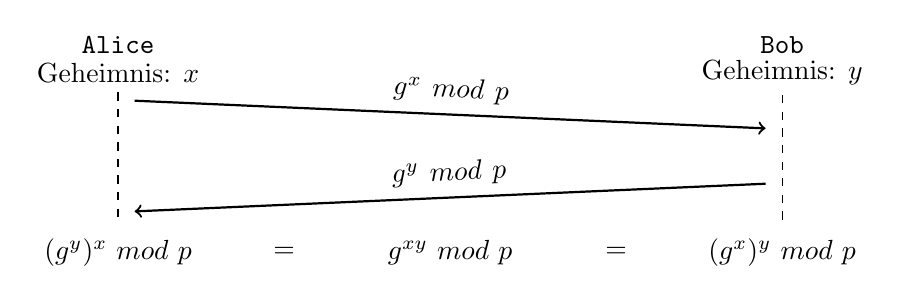
\begin{tikzpicture}[x=2em, y=2em]
				\draw (-6,0) node (Alice) {\texttt{Alice}};
				\draw (-6,-0.5) node (AliceSk) {Geheimnis: $x$};
				\draw (6,0) node (Bob) {\texttt{Bob}};
				\draw (6,-0.5) node (BobSk) {Geheimnis: $y$};
				
				% Lebenslinien
				\draw[dashed] (AliceSk) -- (-6,-3.25);
				\draw[dashed] (BobSk) -- (6,-3.25);
				
				% Pfeile fuer Nachrichten
				\textbf{\draw[->, thick] (-5.7,-1) -- (5.7,-1.5) node[sloped,above,pos=0.5] {$g^x~mod~p$};}
				\textbf{\draw[->, thick] (5.7,-2.5) -- (-5.7,-3) node[sloped,above,pos=0.5] {$g^y~mod~p$};}	
				
				% Beschriftung Ergebnis
				\draw (-6, -3.75) node {$(g^y)^x~mod~p$};
				\draw (-3, -3.75) node {$=$};
				\draw (0, -3.75) node  {$g^{xy}~mod~p$};
				\draw (3, -3.75) node  {$=$};
				\draw (6, -3.75) node  {$(g^x)^y~mod~p$};
			\end{tikzpicture}
		\end{center}
	\end{figure}
	\FloatBarrier
	\item Sicherheit des Verfahrens: Es ist schwierig, den diskreten Logarithmus in einem Primzahlkörper zu berechnen
	\item Vorteile: Keine Infrastruktur notwendig, geheime Zufallszahlen werden nach dem Schlüsselaustausch gelöscht \(\rightarrow\) \textit{Perfect Forward Secrecy}
	\item Nachteile: Anonymer Schlüsselaustausch \(\rightarrow\) keine Authentifizierung der Teilnehmer, MitM-Angriffe möglich, rechenintensiv (und damit anfällig für DoS-Angriffe)
\end{itemize}


\subsection{Bausteine des Schlüsselaustauschs}

\subsubsection{Schlüsselaustauschprotokolle: Bedrohungen}
\begin{itemize}
	\item Man-in-the-Middle-Angriffe: Schlüsselaustausch wird unwissentlich mit dem Angreifer ausgeführt
	\item Replay-Attacken: Wiedereinspielungsangriff von zuvor aufgezeichneten Nachrichten
	\item Denial-of-Service-Angriffen
	\item Downgrade-Attacken: Löschen von starken Algorithmen aus Liste der unterstützten Verfahren zugunsten von veralteten (potentiell schwächeren) Verfahren
	\item Missbräuchliche Schlüsselhinterlegung bei einer vertrauenswürdigen Organisation
\end{itemize}

\subsubsection{Bausteine}
\begin{itemize}
	\item \textbf{Perfect Forward Secrecy}
	\begin{itemize}
		\item Authentifizierung mittels langlebigen Geheimnisses, danach Kommunikation über gesicherten Kanal mit kurzlebigem Sitzungsschlüssel
		\item Ziel: Angreifer kann die Kommunikation auch dann nicht entschlüsseln, wenn er die komplette Kommunikation aufgezeichnet hat und das langlebige Geheimnis kennt (Einbruch in Endsysteme)
		\item Maßnahmen: Sitzungsschlüssel muss von langlebigem Geheimnis unabhängig sein, alle Sitzungsinformationen müssen nach Beendigung der Sitzung gelöscht werden, langlebiges Geheimnis muss periodisch erneuert werden
		\item Beispiel: DH-Austausch mit Authentifizierung. Zusätzlich zu den DH-Parametern werden Signaturen über die Parameter ausgetauscht
	\end{itemize}
	\item \textbf{Schutz der Identitäten}
	\begin{itemize}
		\item Problem: Passiver Angreifer kann Identitäten der Kommunikationspartner abhören
		\item Lösung: Zunächst anonymer DH-Schlüsselaustausch, danach Übertragung der signierten DH-Parameter (setzt vorherige Kenntnis der öffentlichen Schlüssel oder Zertifikate voraus)
	\end{itemize}
	\item \textbf{Dynamische Wahl der Verfahren}
	\begin{itemize}
		\item Dynamische Wahl der genutzten Sicherheitsmechanismn zur Verbesserung der Interoperabilität
		\item Vorteile: Einfache Migration zu kryptographisch stärkeren Verfahren sowie Ausschluss gebrochener Verfahren
		\item Probleme: Komplexität des Protokolls (Wie werden Sicherheitsmechanismen beschrieben und welche Kombinationen sind zulässig?), Downgrade-Angriff
	\end{itemize}
	\item \textbf{Verhinderung von Downgrade-Angriffen\footnote{\url{http://www.golem.de/news/browser-downgrade-angriffe-auf-tls-1309-101305.html}}}
	\begin{itemize}
		\item Ziel des Angreifers: Durch gezielte Verbindungsstörungen dafür sorgen, dass der Client eine Verbindung mit einer älteren Protokollversion durchführt
		\item Anfällig sind beispielsweise Browser, die ältere Protokollversionen als Fallback nutzen: Fast alle gängigen Browser (Firefox, Chrome, Safari, Internet Explorer) führen bei Verbindungsabbrüchen ein Downgrade auf SSLv3 durch
		\item Lösungsansatz: Erkennen von Manipulationsversuchen durch Integritätsschutz (beispielsweise HMAC) aller gesendeten Nachrichten \(\rightarrow\) Integritätsprüfung des gesamten Verlaufs
	\end{itemize}
	\item \textbf{Einschränkung von DoS-Angriffen}
	\begin{itemize}
		\item Ziel: Keine Durchführung von rechenintensiven Operationen, solange nicht klar ist, dass die Absenderadresse nicht gefälscht ist
		\item Möglichkeiten zur Echtheitsprüfung des Anfragenden
		\begin{itemize}
			\item Token/Cookie: Enthält zufällige Informationen des Angefragten. Wird es zurückgesendet, ist mit oher Wahrscheinlichkeit die Absenderadresse nicht gefälscht (beispielsweise durch IP-Spoofing)
			\item Puzzle: Stellen einer rechenintensiven Aufgabe an den Anfragenden. Keine lokale Zustandshaltung beim Angefragten
		\end{itemize}
		\item Konzept: Tokens/Cookies
		\begin{itemize}
			\item Ziel: Serverzustand per Cookie auf Client auslagern \(\rightarrow\) Server muss keinen Zustand pro Anfrage speichern
			\item Schutz der Integrität mittels lokalem Geheimnis. Beispielsweise \(HMAC_K\) über die Zustandsdaten
			\item Anforderungen: Aktualität, Eindeutigkeit, Unverhersagbarkeit, einfache Erzeugung (hoher Aufwand würde DoS-Angriff begünstigen), leichte Verifikation
			\item Erweiterung: Nonce zum Schutz vor Replay-Angriffen
		\end{itemize}
		\item Sitzungswiederaufnahme
		\begin{itemize}
			\item Problem: Initialer Schlüsselaufwand häufig teuer, Verbindungsabbruch bedingt erneuten Schlüsselaustausch
			\item Zustandsbehafteter Ansatz: Zustand nach Schlüsselaustausch wird bei einem Kommunikationspartner gespeichert und kann wiederhergestellt werden (Vgl. TLS-Session-Resumption)
			\item Zustandslos (für Bob): Zustand wird komplett in geschütztes Cookie kodiert und ausgelagert. Kann bei Wiederaufnahme der Sitzung vorgelegt werden (Vgl. Tickets bei Kerberos)
		\end{itemize}
	\end{itemize}
\end{itemize}


\subsection{Digitale Zertifikate}
\begin{itemize}
	\item Idee: Authentifizierung von Sachverhalte, die man nicht selbst überprüfen kann, durch vertrauenswürdige Dritte
	\item Sichere Zuordnung von öffentlichen Schlüsseln und Identitäten der Kommunikationspartner
	\item Lösung: Verwendung von Zertifikaten. Authentifizierung hier durch vertrauenswürdige Dritte und Bestätigung durch digitale Signatur (Vgl. Personalauswand/Reisepass)
	\item Probleme: Anbieter erfährt wer mit wem kommuniziert; Single-Point-of-Failure; schlechte Skalierung
	\item \textbf{Klassifizierung von Zertifikaten}
	\begin{itemize}
		\item ID-Zertifikat: Bindet öffentlichen Schlüssel an eindeutige Identität (Verwendung beispielsweise bei S/MIME)
		\item Attributzertifikat: Bindet Attribute an eindeutige Identität (Verwendung beispielsweise beim elektronischen Führerschein)
	\end{itemize}
\end{itemize}



\section{Vertrauensmodelle}

\subsection{Motivation}
\begin{itemize}
	\item Idee: Absichern von asymmetrisch verschlüsselter Kommunikation mit Hilfe von digitalen Zertifikaten. Zentrale Frage: Wer erstellt die vertrauenswürdige Instanz?
	\item \textbf{Neue Probleme}
	\begin{itemize}
		\item Vertrauen in die CA, bzw. deren Integrität (und in die Gewissenhaftigkeit der Identitätsprüfung)
		\item Gültigkeit der Zertifikate
		\item Authentizität des öffentlichen Schlüssels der CA
		\item Konflikte, wenn mehrere CAs die selbe Entität signieren
		\item Wer steht an der Spitze der CA(-Kette)?
	\end{itemize}
	\item \textbf{Widerruf digitaler Zertifikate}
	\begin{itemize}
		\item Widerruf manchmal notwendig, beispielsweise wenn der private Schlüssel verloren gegangen oder korrumpiert worden ist
		\item CA stellt signierte \textit{Certificate Revocation List} zur Verfügung
	\end{itemize}
\end{itemize}


\subsection{Infrastrukturen}

\subsubsection{Public Key Infrastructure (PKI)}
\begin{itemize}
	\item Zentrale Infrastructur zum Management von ID-Zertifikaten \(\rightarrow\) ermöglicht Authentifizierung öffentlicher Schlüssel
	\item \textbf{Anforderungen}
	\begin{itemize}
		\item Vertrauenswürdigkeit
		\item Sicherheit interner Abläufe (Dokumentation soll Vertrauenswürdigkeit erhöhen) und der Signaturschlüssel der CA
		\item Effiziens, Skalierbarkeit, Komfort für den Benutzer
	\end{itemize}
	\item \textbf{Elemente}
	\begin{itemize}
		\item Benutzer: Person oder Serverinstanz
		\item Registration Authority (RA): Implementiert die administrativen Aspekte der PKI, Schnittstelle zwischen Benutzer und CA. I.d.R. offline
		\item Certification Authority (CA): Führt die Zertifizierungen durch und ist für den Schutz der eigenen privaten Schlüssel zuständig
		\item Verzeichnisdienst (Directory): Verwaltet die Zertifikate (beispielsweise LDAP) und publiziert die Widerrufslisten
	\end{itemize}
\end{itemize}

\subsubsection{Privilege Management Infrastructure (PMI)}
\begin{itemize}
	\item Access Control List (ACL): Definiert, wer auf eine Ressource zugreifen kann
	\item \textbf{Methoden zur Autorisierung}
	\begin{itemize}
		\item Discretionary Access Control: Individuelle, feingranulare Rechtevergabe pro Benutzer
		\item Mandantory Access Control: Benutzer werden klassifiziert und bekommen klassenbezogene Zugriffsrechte
		\item (Hierachical) Role-based Access Control: Benutzer werden Rollen zugewiesen, die über entsprechende Rollen verfügen. Ggf. vererbt
		\item Attributzertifikat: Attestieren Identitäten ein bestimmtes Privileg (als Attribut implementiert). Zeitlich beschränkt und kann per CRL zurückgerufen werden
	\end{itemize}
	\item PMIs realisieren Autorisierung auf Basis von Attributzertifikaten. Aufbau mit PKI vergleichbar
	\item \textbf{Aufbau einer PMI}
	\begin{itemize}
		\item Attribute Authority (AA, vgl. CA): vergibt Zugriffsrechte und zertifiziert diese
		\item Source of Authority (SOA, vgl. Root CA): Oberste Attribute Autority, zertifiziert alle weiteren Privilegien
	\end{itemize}
\end{itemize}


\subsection{Vertrauen/Vertrauensmodelle}
\begin{itemize}
	\item Vertrauen: Normal im Alltagsleben, subjektiv, unscharf, gerichten, kontextgebunden, risikoabhängig, etc.
	\item \textbf{Vertrauensmodell (Trust Model)}
	\begin{itemize}
		\item Beschreibt, welchen Zertifikaten ein Benutzer trauen kann;, wie Vertrauen hergestellt wird und wie dieses Verhalten eingeschränkt/kontrolliert werden kann
		\item Vertrauensanker (Trust Anchor): Ausgangspunkt einer Zertifizierungskette (beispielsweise eine Root CA)
		\item Modelle
		\begin{itemize}
			\item Single-CA
			\begin{itemize}
				\item Eine CA erstellt alle Zertifikate
				\item Vorteil: Nur ein Vertrauensanker erleicht die Validierung
				\item Nachteile: Globales Vertrauen notwendig, Monopolstellung, Kompromittierung des CA-Schlüssels hat globale Konsquenzen, Skalierung, Single-Point-of-Failure
			\end{itemize}
			\item Oligarchie von CAs
			\begin{itemize}
				\item Zertifizierung durch mehrere CAs (Distributed Trust Architecture)
				\item Vorteile: Keine Monopolstellung, Kompromittierung hat begrenzte Auwirkung
				\item Nachteile: Initiale Prüfung sowie Validierung durch mehrere CAs, mehrere CA-Schlüssel müssen geschützt werden
			\end{itemize}
		\end{itemize}
		\item Transitivität von Vertrauen
		\begin{itemize}
			\item Notwendig für komplexere Vertrauensmodelle
			\item Mathematische Definition: Wenn \(A\) Vertrauen in \(B\) (und dessen Zertifizierungen) hat und \(B\) Vertrauen in \(C\) (und dessen Zertifizierungen), so kann \(A\) auch Vertrauen in \(C\) (und dessen Zertifizierungen) haben
			\item Anstatt einem einzigen Zertifikat zu vertrauen werden jetzt Zertifikatsketten zwischen Vertrauensanker und Endpunkt aufgebaut und jede Stufe separat validiert
		\end{itemize}
		\item Transitive Modelle
		\begin{itemize}
			\item Oligarchie von CAs mit Delegierung
			\begin{itemize}
				\item CAs können untergeordnete CAs (Sub-CAs) einsetzen. Dadurch ergeben sich Zertifikatsketten
				\item Vorteile: Kompromittierung von CA-Schlüsseln hat begrenzten Wirkungsbereich, Skalierung
				\item Nachteile: Höhere CA-Schlüsselzahl notwendig, Validierung aufwendiger
			\end{itemize}
			\item Top-Down
			\begin{itemize}
				\item Single-CA mit Delegation und Einschränkunge der Delegation auf Teilbereiche eines hierarchischen Namensraums (beispielsweise DNS oder X.500)
				\item Vorteile: Kompromittierung von CA-Schlüsseln hat begrenzten Wirkungsbereich, Skalierung, kontrollierte Delegation
				\item Nachteile: Höhere CA-Schlüsselzahl notwendig, Validierung aufwendiger, immer Validierung des ganzen Pfades
			\end{itemize}
			\item Anarchie
			\begin{itemize}
				\item Jeder Benutzer fungiert als CA und je nach Bedarf (transitiv) eingesetzt werden (beispielsweise PGP)
				\item Vorteil: Auswirkung bei Kompromittierung beschränkt
				\item Nachteile: Alle Schlüssel sind CA-Schlüssel, Skalierbarkeit (hohe Anzahl Schlüssel \(\rightarrow\) Pfadfindung schwer, da nicht eindeutig), keine einheitliche Zertifizierungspolitik (Transitivität von Vertrauen problematisch), Zertifizierungen schwer kontrollierbar/einschränkbar
			\end{itemize}
		\end{itemize}
	\end{itemize}
\end{itemize}


\subsection{Beispielprotokolle}

\subsubsection{X.509}
\begin{itemize}
	\item Bekannster und verbreitetster Standard für Zertifikate
	\item Erweiterungsmöglichkeit duch optionale Parameter; auch als Attributzertifikat verwendbar
	\item Aktive Nutzung: SSL/TLS, S/MIME, IPsec, etc.
	\item Hierarchisches Namensschema: \textit{Distinguished Name} setzt sich aus mehreren Attributen zusammen (beispielsweise Land, Bundestaat, Stadt, etc.)
	\item \textbf{Aufbau}
	\begin{itemize}
		\item Subject: Besitzer des Zertifikats
		\item Issuer: ID des Erzeugers des Zertifikats, nächster Schritt in der Zertifikatskette
		\item Version/Seriennummer/Signaturalgorithmus/Gültigkeit
		\item Erweiterungen
	\end{itemize}
	\item \textbf{Wichtige Erweiterungen}
	\begin{itemize}
		\item Verwendung mehrerer Schlüssel: Mehrere Erweiterungsmöglichkeiten zur Verwendung weiterer Schlüssel
		\item Alternativnamen für Subjekte: X.500-Namen wenig verbreitet, daher Verwendung von \textit{Subject-Issuer Alternative Names}. So können auch beispielsweise IP-Adressen, E-Mail-Adressen, Domains, etc. verwendet werden
	\end{itemize}
	\item \textbf{Extended Validation}
	\begin{itemize}
		\item Ziel: Höheres Maß an Vertrauen durch erweiterte Überprüfung
		\item Richtlinien mit technischen/organisatorischen Anforderungen
		\item Zertifikate enthalten \textit{certificatePolicies}-Erweiterungen (\texttt{OID} der Policy für EV-Zertifikate sowie URL zum \textit{Certification Practice Statement})
	\end{itemize}
	\item \textbf{PKI-Unfälle}
	\begin{itemize}
		\item Immer wieder Einbrüche bei bekannten PKI-Betreibern
		\item Microsoft Windows kann einige eigene Zertifikate nicht auf Widerruf prüfen (CRL nicht implementiert) \(\rightarrow\) schwächstes Glied in der Kette bestimmt die Gesamtsicherheit
	\end{itemize}
\end{itemize}

\subsubsection{OCSP/SCVP}
\begin{itemize}
	\item \textbf{Online Certificate Status protocol (OCSP)}
	\begin{itemize}
		\item Erster Ansatz zur Onlineprüfung von Zertifikaten auf Widerruf mittels einfachem Frage-Antwort-Schema
		\item Erweiterung im Zertifikat zur Spezifizierung von Respondern und des zu verwendenden Protokolls (beispielsweise LDAP/HTTP). Responder wird ebenfalls signiert
		\item Einschränkungen
		\begin{itemize}
			\item Antwortet nur in Bezug auf Widerruf. Keine Prüfung von Verwendungszweck oder zeitliche Gültigkeit
			\item Schlechte Skalierung beim Responder, da Antwort immer signiert wird (Vgl.: Bei CRLs muss nur einmal signiert werden, bei OCSP bei jeder Anfrage)
			\item Verringert Clientaufwand zur Zertifikatsprüfung kaum
			\item Angreifer kann OSCP-Anfrage eventuell blockieren
		\end{itemize}
	\end{itemize}
	\item \textbf{Server-based Certificate Validation Protocol (SCVP)}
	\begin{itemize}
		\item Soll Clients ein partielles bis vollständiges Auslagern der Zertifikatsprüfung ermöglichen
		\item Teilweise Auslagerung
		\begin{itemize}
			\item Auslagerung des Aufbaus der Zertifikatskette (Delegated Path Discovery)
			\item Client führt die Püfung der Zertifikatskette selbst durch \(\rightarrow\) kein vertrauenswürdiger Server erforderlich
		\end{itemize}
		\item Vollständige Auslagerung
		\begin{itemize}
			\item Auslagerung der kompletten Zertifikatsprüfung (Delegated Path Validation)
			\item Vertrauenswürdiger Server erforderlich
		\end{itemize}
	\end{itemize}
\end{itemize}



\section{Authentifizierung}

\subsection{Authentifizierung von Nutzern}

\subsubsection{Password Authentication Protocol (PAP)}
\begin{itemize}
	\item Idee: Nutzer authentifiziert sich mittels Netzerkennung und dazugehörigem Passwort bei Ressource
	\item Schwächen: Übertragung im Klartext (MitM- oder Replay-Angriff möglich), Client ist Initiator (DoS-Angriff möglich), Ressource hat Zugriff auf das Klartext-Kennwort
	\item Praktikabel über zuvor aufgebauten sicheren Kanal mit authentifizierung der Ressource
\end{itemize}

\subsubsection{Challenge Handshake Authentication Protocol (CHAP)}
\begin{itemize}
	\item Client schickt einen gehashte Kombination aus Passwort und zuvor angefragter und erhaltener Challenge an den Server
	\item Vorteile gegenüber PAP: Passwort wird nicht im Klartext übertragen, bei guter Challenge kein Replay-Angriff möglich, Hash-Algorithmus frei wählbar
	\item Nachteil: Passwort weiterhin im Klartext gespeichert
	\item Paxisbeispiel MS-CHAPv2 von Microsoft: Client schickt DES-verschlüsselte Kombination aus Challenge und gehashtem Passwort an den Server. DES allerdings gebrochen, daher MS-CHAPv2 nur noch über gesicherten Kanal verwendbar
\end{itemize}

\subsubsection{S/Key}
\begin{itemize}
	\item Ziel: Verhinderung von Replay-Angriffen, Vermeidung von Passwörtern auf Ressource
	\item Idee: Hashkette
	\item \textbf{Vorbereitungen}
	\begin{itemize}
		\item Client generiert Einmal-Kennwörter nach dem Schema: \(S_0=H(Passwort+Seed),S_1=H(S_0),...,S_n=H(S_{n-1})\)
		\item Ressource speichert das Paar \(\{n,S_n\}\), Client speichert alle Einmalkennwörter \(S_1,...S_n\)
	\end{itemize}
	\item \textbf{Ablauf}
	\begin{itemize}
		\item Server schickt Challenge \(n\) an den Client
		\item Client sendet \(S_{n-1}\) an den Server
		\item Server verifiziert mittels \(H(S_{n-1})=S_n\), bestätigt/lehnt ab und speichert \(\{n-1,S_{n-1}\}\) für die nächste Authentifizierung
		\item Wiederhole bis alle Passwörter aufgebraucht sind, danach Neugeneration
	\end{itemize}
\end{itemize}

\subsubsection{Extensible Authentication Protocol (EAP)}
\begin{itemize}
	\item Idee: Generisches Protokoll mit Unterstützung beliebiger Module zur Authentifizierung
	\item \textbf{Ablauf (dynamisch anpassbar)}
	\begin{itemize}
		\item Ressource sendet nach client-initiierter Authentifizierungsanfrage mehrere Anfragen an den Client: Frage nach ID/Angebot von Modulen/Challenge
		\item Client lehnt ab oder sendet die angeforderten Daten zurück
		\item Ressource anwortet mit (Miss-)Erfolg oder stellt weitere Fragen
	\end{itemize}
	\item Beispielmodule: MD5-Challenge, Generic Token Card (hardware-basiert, sonst wie CHAP), One-Time Passwort
	\item Verpflichtende Module: Identity (ermittelt die ID des zu authentifizierdenden Clients), Notification (übertragen einer Nachricht an den CLient, welche dieser bestätigen muss), NAK (Ablehnung einer Antwort)
	\item Viele (auch kommerzielle) Module standardisiert
\end{itemize}


\subsection{Authentifizierungsdienste}
Zentraler Dienst zur Authentifizierung (AS) im Unternehmen gewünscht, um Mehrfachpflege von Benutzeraccounts zu vermeiden.

\subsubsection{RADIUS}
\begin{itemize}
	\item Aufgaben: Transport von Authentifizierungsdaten, Proxyfunktion zum Weiterleiten an anderen AS (Roaming)
	\item Ursprünglich nur Unterstützung von PAP und CHAP, mittlerweile auch von EAP
	\item Klassisches Client-Server-Protokoll, arbeitet zwischen Ressource und AS in Anwendungungsschicht oberhalb von UDP
	\item \textbf{Rollen}
	\begin{itemize}
		\item Client (Supplicant): Initiiert die Authentifizierung bei der Ressource
		\item Ressource (RADIUS-Client): Handelt Authentifizierungsverfahren mit Client aus und kommuniziert mit AS
		\item AS (RADIUS-Server): Nimmt die Authentifizierungsanfrage entgegen, authentifiziert und autorisiert den Benutzer und gibt die Antwort zurück. Leitet die Anfrage ggf. zu betreffendem AS weiter (Roaming)
	\end{itemize}
	\item \textbf{Authentifizierung mit EAP}
	\begin{itemize}
		\item Problemstellung: Ressource authentifiziert Client meist über EAP (beispielsweise PPP, PPPoE, 802.1X). Dazu müssen allerdings Daten aufwendig zwischen EAP-Paketen und RADIUS-Attributen kopiert/umgesetzt werden
		\item Idee/Lösungsansatz: Verwenden von RADIUS-Attribut "`EAP-Mesage"' zur Übersetzungsvermeidung in einzelne RADIUS-Attribute
	\end{itemize}
	\item \textbf{Roaming}
	\begin{itemize}
		\item Betrieb von mehreren RADIUS-Servern
		\item Erster AS fungiert als Proxy für weitere AS und leitet alle Nachrichten weiter
	\end{itemize}
	\item \textbf{Sicherheitsbetrachtungen}
	\begin{itemize}
		\item Schutzziele (Ressource \(\leftrightarrow\) AS): Vertraulichkeit/Integrität der Nachrichten sowie Authentizität der Kommunikationspartner
		\item Umsetzung bei RADIUS: Gemeinsames (16 Byte langes) Geheimnis zwischen Ressource und AS
		\item Fazit
		\begin{itemize}
			\item Sicherheit steht und fällt mit dem Shared Secret. Dieses muss manuell verteilt werden und fehlt beim Roaming \(\rightarrow\) nicht alle Daten sind auf dem Kommunikationsweg geschützt
			\item Sicherheit allgemein unzureichend, schwache Sicherung der Schutzziele sowie schwacher Schutz gegen Wiederholungsangriffe
			\item Lösung: Verwenung von TLS (oberhalb von TCP) zur Sicherstellung der Schutzziele
		\end{itemize}
	\end{itemize}
\end{itemize}

\subsubsection{Diamter}
\begin{itemize}
	\item Nachfolger von RADIUS, allerdings nicht vollständig abwärtskompatibel
	\item Vorteile gegenüber RADIUS: Verlässliche Transportprotokolle (TCP oder SCTP), Fokus auf Sicherheit (Verpflichtender Einsatz von IPsec oder TLS), bessere Roaming-Unterstützung, leichte Erweiterbarkeit, Basisunterstützung für Accounting
	\item \textbf{Diameter Application}
	\begin{itemize}
		\item Spezifiziert Framework für Anwendungen: Dienste/Protokolle/Mobile IP/Accounting sowie Ressourcen und AS-Funktionalität
		\item Applikationen können Diamter-Funktionalität nutzen, beispielsweise Server-/Proxykomponenten, Verbindungsaufbau, Sitzngsmanagement, Kommunikationssicherheit
	\end{itemize}
	\item \textbf{Sicherheitsbetrachtung}
	\begin{itemize}
		\item Sicherheit von Anfang an im Fokus: verwendung von IPsec vorgschrieben, Server muss zusätzlich TLS unterstützen
		\item Hoher Schutz der Kommunikation zwischen Ressource und AS
		\item Kommunikation zwischen Client und Ressource muss weiterhin zusätzlich gesichert werden
	\end{itemize}
\end{itemize}



\section{Kerberos}
\begin{itemize}
	\item Verteilter Authentifizierungsdienst für Benutzer und Server in (un-)geschützten Netzwerken
	\item SingleSignOn innerhalb der Domäne
	\item \textbf{Komponenten}
	\begin{itemize}
		\item \textit{Authentication Server} (AS) zur Authentifizierung der Benutzer sowie zur Ausstellung von Authentifizierungstokens (\textit{Ticket-Granting-Ticket}: TGT)
		\item \textit{Ticket Granting Server} (TGS): Ressourcen-Zugangs-Server zur Autorisierung des Ressourcen-Zugriffs mit gültigem TGT. Ausstellung von Zugangsberechtigungen (\textit{Tickets})
		\item Benutzerdaten zur Speicherung der \textit{Master-Secrets} aller Benutzer und Ressourcen
		\item AS und TGS bilden \textit{Kerberos Distribution Center} (KDC)
	\end{itemize}
	\item \textbf{Ablauf einer Anmeldung}
	\begin{enumerate}
		\item Anmeldung beim AS: Client erhält TGT
		\item Ressourcenanforderung: Autorisierung durch TGT. Client erhält Ticket für die entsprechende Ressource
		\item Kommunikation mit der Ressource. Zugriffskontrolle erfolgt durch die Ressource
	\end{enumerate}
	\item \textbf{Anmeldung am Netz}
	\begin{itemize}
		\item Übertragen des Benutzernames im Klartext zum KDC (Angreifer kann Identität des Benutzers abhören). Nonce zum Schutz vor Replay-Attacken (\texttt{AS\_REQ})
		\item Antwort vom Server (\texttt{AS\_REP}) mit dem Master-Secret des Benutzers verschlüsselt (verschiedene Verfahren wie beispielsweise AES unterstützt)
	\end{itemize}
	\item \textbf{Offline-Password-Guessing-Angriff}
	\begin{itemize}
		\item Ziel: Erlangen des Benutzerpassworts
		\item Vorgehen: Abhören von \texttt{AS\_REQ} und \texttt{AS\_REP}, anschließend Wörtbuchangriff zur Ermittlung des Passworts
		\item Bei (veraltetem) Kerberos v4: Aktiver Angriff durch Generierung von \texttt{AS\_REQ}-Anfragen für beliebige Nutzer
		\item Optionaler Schutz in Kerberos v5 integriert: Zusätzlich aktueller Zeitstempel mit Master-Key des Client verschlüsselt in \texttt{AS\_REQ} enthalten. Brute-Force-Angriffe weiterhin möglich
	\end{itemize}
	\item Optional Netzwerkadressen der Clients in jedem Ticket: Keine Weitergabe von Tickets \(\rightarrow\) schützt vor Ticketdiebstahl. IP-Spoofing allerdings unkompliziert möglich, funktioniert nicht bei NAT
	\item \textbf{Schlüssel-Server für große Netze}
	\begin{itemize}
		\item Einzelner KDC ist Single-Point-of-Failure \(\rightarrow\) Replizieren des Schlüssel-Servers
		\item Gliederung des Netzwerk in Domänen (Realms). Einzelner KDC kennt nicht mehr alle Master-Secrets
		\item Replizierte Schlüssel-Server
		\begin{itemize}
			\item Eine Master-Copy der Benutzerdatenbank mit mehreren Read-only-Slave-KDCs. Alle Änderungen nur auf der Master-Copy
			\item Auch bei Ausfall des Master-KDC ist die Nutzung des Netzes weiterhin möglich, lediglich Änderungen fallen aus
			\item Periodisches Abfragen der Slaves (oder per Kommando). Updates verschlüsselt und mit MAC versehen
			\item Passwortänderung problematisch
			\begin{itemize}
				\item Passwort muss jederzeit änderbar sein
				\item Problem (I): Bereits ausgestellte Tickets sind mit dem alten Passwort verschlüsselt
				\item Lösung (I): Speicherung mehrerer Schlüsselversionen sowie Ergänzen der Tickets um die Version
				\item Problem (II): Replizieren des KDCs. Bei periodischem Verteilen eventuell noch das alte Kennwort auf dem Slave \(rightarrow\) altes Passwort weiterhin gültig \(\rightarrow\) Verwirrung des Benutzers
			\end{itemize}
		\end{itemize}
		\item Rechteübertragung % TODO!
		\begin{itemize}
			\item Erst ab Kerberos v5 möglich
		\end{itemize}
		\item Domänen (Realms)
		\begin{itemize}
			\item Administrative Aufteilung pro Realm: Eigene Benutzerdatenbank, Replizierung, KDCs einer Domäne beisitzen das selbe KDC-Master-Secret
			\item Inter-Domänen-Authentifizierung zur Nutzung von Ressourcen einer anderen Domäne. Autorisierung durch den KDC der anderen Domäne. KDC kann hierzu als Client eines anderen KDC registriert sein
			\item Mehrstufige Domänen durch Verkettung von Inter-Domänen-Tickets möglich. KDC registriert sich hierzu als Client bei KDC der Vaterdomäne
		\end{itemize}
	\end{itemize}
	\item \textbf{Zusammenfassung}
	\begin{itemize}
		\item SSO-Netzwerk; Tickets mit Cookie-Prinzip; Übertragung von Rechten möglich; KDC als Single-Point-of-Failure (Replizierung, Mehrstufigkeit)
		\item Vorteile: Nur ein Passwort; sichere, netzwerkweite Authentifizierung; basiert fast ausschließlich auf symmetrische Verfahren
		\item Nachteile: Kompromittierung des Master-Secrets des KDC legt alle Master-Secrets der Clients offen; alle Ressourcen müssen angepasst sein ("`kerberized"'); enge Synchronisation der Systemuhren notwendig
	\end{itemize}
\end{itemize}



\section{Zugangsschutz}
\begin{itemize}
	\item \textbf{Bestandteile}
	\begin{itemize}
		\item Network Access Server (NAS): Einwahl-/Verbindungspunkt für Nutzer. Blockiert zunächst Zugriffe der Nutzer und wartet auf Authentifizierung und Autorisierung
		\item Authentication Server (AS): Speichert Informationen zum Nutzer und nimmt Authentifizierungsanfragen entgegen
	\end{itemize}
	\item \textbf{Netzzugangstechniken}
	\begin{itemize}
		\item Dediziertes, physisches Medium: Hier direkte Punkt-zu-Punkt-Verbindungen wie POTS, ISDN oder LAN. Angriffe schwierig, brauchen physischen Zugriff
		\begin{itemize}
			\item Einwahlverbindung per Point-to-Point Protokoll (PPP). Unterteilt in:
			\begin{itemize}
				\item \textit{Link Configuration Protocol} (LCP) zur Authentifizierung auf Schicht 2
				\item \textit{Network Configuration Protocol} (NPC) zur Einrichtung von Schicht 3 (beispielsweise IP)
			\end{itemize}
			\item Entwickelt für dediziertes, physisches Medium und unterstützt verschiedene Transportptotokolle. Häufiger Einsatz bei ISPs
			\item Keine Sicherheit auf dem Übertragungsweg zwischen Supplicant und NAS, keine Sicherheit für anschließende Kommunikation
			\item Annahme: Angriffe schwierig, da direkter Zugriff benötigt (und dieser ist nicht vorhanden)
			\item PPP und DSL: PPP over Ethernet (PPPoE)
			\begin{itemize}
				\item Ethernet als Anschlusstechnologie zur Kosteneinsparung der Provider (geteiltes Medium: Punkt-zu-Multipunkt). Allerdings fehlende Funktionalität in Ethernet wie Authentifizierung, Aushandling von Optionen, Accounting
				\item \textit{Broadband Remote Access Server} (BRAS) als Gegenstelle der Supplicants (übernimmt die Rolle des NAS)
				\item Problem: Auffinden der richtigen Gegenstelle (welche MAC hat der BRAS)
				\item Bei PPPoE werden PPP-Pakete in Ethernet-Dateneinheiten übertragen \(\rightarrow\) Authentifizierung via PPP
				\item PPPoE-Discovery zum Finden der NAS-Gegenstelle
				\item Auch PPPoE verwendet keine zusätzlichen Sicherheitsfeatures
			\end{itemize}
		\end{itemize}
		\item Geteiltes Medium: Drahtgebunde Punkt-zu-Mehrpunkt-Verbindungen (Ethernet) wie DSL, DOCSIS (Kabelnetz) oder LAN (Bus). Angriffe für Insider leicht (ARP-/IP-Spoofing), externe Angreifer benötigen zunächst Mediumzugriff
		\begin{itemize}
			\item Punkt-zu-Punkt-Verbdinung mittels LAN-Kabel zum NAS (Port Access Entity - PAE, hier: Switch) via Ethernet auf Schicht 2 (IEEE 802.3)
			\item Port-basierte Authentifizierung und Autorisierung zum Schutz vor illegitimer Nutzung des LAN
			\item EAP zur Authentifizierung (EAP over LAN)
			\begin{itemize}
				\item Ethernat zwischen Supplicant und Authenticator/NAS. Transport von EAP über Ethernet
				\item Netzwerkstack: Ethernet \(\rightarrow\) EAPoL-Dateneinheit \(\rightarrow\) EAP-Dateneinheit
				\item Sicherheitsbetrachtung: Einmal authentifizierter Port kann mittels Netzwerk-Hub "`entführt"' werden. Keine Sicherheit auf dem Übertragungsweg und während der anschließenden Kommunikation. Annahme: Angreifer hat keinen Zugriff auf das Medium
			\end{itemize}
		\end{itemize}
		\item Broadcast Medium: Hier drahtlose Punkt-zu-Mehrpunktverbindungen für alle in Empfangsreichwerte. Beispielsweise WLAN. Angriffe für Insider einfach, externe Angreifer müssen nur in Empfangsreichweite sein
		\begin{itemize}
			\item Boradcast Medium mit Kommunikation über Luftschnittstelle. Jede gesendete Nachricht wird an alle Teilnehmer weitergeleitet \(\rightarrow\) Angriffe leicht möglich
			\item Zugangsverfahren
			\begin{enumerate}
				\item WEP (gebrochen)
				\begin{itemize}
					\item Verwendung der Stromchiffre RC4. Wahlweise Open-System oder Authentifizierung via PSK
					\item Lediglich Gruppenauthentifizierung mit gemeinsamen Schlüssel, keine Authentifizierung einzelner User
				\end{itemize}
				\item WPA (gebrochen)
				\begin{itemize}
					\item Ab 2003 Alternative zu gebrochenem WEP notwendig
					\item Temporal Key Integrity Protocal (TKIP) sowie individuelle Sitzungsschlüssel auf Basis von RC4 zur Verschlüsselung und Integrität
					\item Neben gemeinsamem Sitzungsschlüssel auch pro-Benutzer-Zugänge möglich (802.1X, Authentifizierung via RADIUS-Server)
					\item Probleme: Keine starken Kryptomechanismen. Verschlüsselung/Authentifizierung/integritätssicherung gilt als gebrochen
				\end{itemize}
				\item WPA2 mit PSK (ungebrochen, derzeit bester Angriff: PSK raten)
				\begin{itemize}
					\item Vollständige Umsetzung von IEEE 802.11i (Robust Security Network): Authentifizierung via PSK ("`personal"') oder 802.1X ("`enterprise"'), Verschlüsselung zwingend AES-CCMP (Counter-Mode-with-Cypther-Block-Chaining)
					\item Bewertung WPA2-Personal: Authentifizierung von Nutzern sowie Schutz der Kommunikation zwischen Supplicant und NAS, allerdings Authentifizierung nur auf Basis von Gruppenzugehörigkeit \(\rightarrow\) schwierig einzelne Nutzer zu identifizieren (beispielsweise bei Rechtsstreitigkeiten)
					\item Bewertung von WPA-Enterprise: Löst die Probleme des Personal-Modus, verwendet etablierte Standards
				\end{itemize}
			\end{enumerate}
		\end{itemize}
		\item Netzwerkübergreifend (beispielsweise über das Internet): Supplicant ist nicht im gleichen lokalen Netz wie NAS (VPN). Angriffe leicht, da viele weitervermittelnde Netzwerke
		\begin{itemize}
			\item Ziel: Gesicherten Zugriff auf Zielnetzwerk mit Zugriffs- und Übertragungsschutz
			\item Nutzung von PPP-Authentifizierung über IP/UDP
			\item Implementierungen: Point-to-Point-Protocol von Microsoft (verwendet MS-CHAPv2, gilt als gebrochen) oder Layer-2-Tunneling-Protocol (L2TP)
			\item Netzwerkstack: IP \(\rightarrow\) UDP \(\rightarrow\) PPP \(\rightarrow\) Schicht 3 \(\rightarrow\) Schicht 4
			\item L2TP: Virtuelle Punkt-zu-Punkt-Verbindung via UDP. Bietet keine Vertraulichkeit, daher meist in Kombination mit IPsec verwendet. Nutzt PPP zur Einwahl ins Zielnetzwerk und zur Authentifizierung (beispielsweise mittels EAP)
			\item OpenVPN mit TLS: Betriebssystem-unabhängige VPN-Einwahl mit guter Konnektivität durch Firewalls und NATs. Authentifizierung beispielsweise mittels PSK oder Benutzername und Kennwort. Darüber hinaus Verwendung von Zertifikaten
		\end{itemize}
	\end{itemize}
	\item \textbf{Beispielszenario: Eduroam}
	\begin{itemize}
		\item Föderativer Ansatz für Internetzugang über Universitäten für globalen Internetzugang von Studenten/Mitarbeitern. Dezentrale Speicherung \(\rightarrow\) Authentifizierung der Nutzer über die jeweilige Universität
		\item Schutzziele: Schutz auf Schicht 2 sowie gegenseitige Authentifizierung von Supplicant und AS
		\item Aufbau
		\begin{itemize}
			\item Eindeutige, globale Identifikation der Benutzer (beispielsweise \texttt{benutzer@student.kit.edu})
			\item Aufteilung in Authentifizierungsdomänen (Realms): Jede teilnehmende Universität stellt eigenen AS (Identitätsprovider, RADIUS-Server)
			\item Hierarchischer Zusammenschluss je Land zu einer Föderation sowie Zusammenschloss der Föderationen zu entsprechenden Konföderationen (Europa, Asien-Pazifik, USA, Kanada, etc.)
			\item Roaming über hierarchisches RADIUS-Netzwerk
			\item Probleme bisher:
			\begin{itemize}
				\item Schutz nur jeweils zwischen Supplicant/NAS, NAS/AS, AS/AS. Zwischensysteme können Daten abhören/manipulieren \(\rightarrow\) kein Schutz auf dem kompletten Kommunikationsweg zwischen Supplicant und Heimat-AS
				\item NAS erfährt den konkreten Benutzernamen \(\rightarrow\) kein Schutz der Identität
				\item Keine Authentifizierung des Heimt-AS
			\end{itemize}
			\item Zusätzliche Probleme bei 802.1X und WLAN
			\begin{itemize}
				\item Passiver Angriff durch Mitschneiden der initialen Identitätsdaten immer möglich
				\item Aktive Angriffe wie MitM-Angriffe während der Authentifizierung oder Fälschen von Dateneinheiten möglich
			\end{itemize}
			\item Schutz des Authentifizierungsverkehrs
			\begin{itemize}
				\item Protected-EAP (PEAP): Proprietäres Protokoll von Microsoft/Cisco
				\item EAP-Tunneled-TLS (EAP-TTLS): IETF-standardisiert. Zunächst Aufbau einer gesicherten TLS-Verbindung mit anonymem Supplicant, danach Authentifizierung über sicheren Tunnel. Nachteile: Ob AS-Zertifikat validiert wird hängt vom Supplicant ab, problematisch bei zurückgerufenen Zertifikaten 
			\end{itemize}
		\end{itemize}
	\end{itemize}
\end{itemize}



\section{IPsec}

\subsection{Einführung}
\begin{itemize}
	\item \textbf{Motivation}
	\begin{itemize}
		\item Internet-Protocol (IP) bietet einen nur unzuverlässigen Ende-zu-Ende Dienst
		\item Mögliche Angriffe: Eavesdropping, IP-Spoofing, MitM-Angriffe, Replay-Angriffe \(\rightarrow\) Schutzziele nicht gewährleistet
	\end{itemize}
	\item \textbf{Überblick}
	\begin{itemize}
		\item Ziel: Umsetzung von Schutzzielen für den Verkehr auf Schicht 3, unabhängig vom Transportprotokoll
		\item Nutzung durch alle oberhalb von IP angesiedelten Protokolle sowie IP selbst
	\end{itemize}
	\item \textbf{Einsatzszenario}
	\begin{itemize}
		\item Häufiger Einsatz als VPN, beispielsweise in Unternehmen mit verschiedenen Standorten, die über das Internet kommunizieren
	\end{itemize}
	\item \textbf{Grundlegender Aufbau}
	\begin{itemize}
		\item Wesentliche Komponenten: Schlüsselaustausch (Internet Key Exchange - IKE) und Protokolle zur sicheren Kommunikation (Authentication Header - AH oder Encapsulating Security Payload - ESP)
		\item Entwurfsentscheidung: Entkopplung von Schlüsselaustausch und Sicherung
	\end{itemize}
\end{itemize}


\subsection{Security Policy}
\begin{itemize}
	\item \textbf{Sicherheitsassoziation}
	\begin{itemize}
		\item Flexibilität: Teilnehmer können entscheiden welche Sicherheitsanforderungen an einen IP-Strom gestellt werden
		\item Security-Association (SA): Unidirektionale Verbindung zwischen zwei IP-Instanzen. Generell zwischen allen Verbindungen möglich
	\end{itemize}
	\item \textbf{SAD und SPD}
	\begin{itemize}
		\item Security Associaten Database (SAD): Hält Parameter aktiver gesicherter IP-Datenströme
		\item Security Policy Database (SPD): Enthält Richtlinien nach denen der Verkehr zu schützen ist. Zu sendende Dateneinheiten werden gemäß SPD auf SA abgebildet. Besteht aus einer Tabelle, die beschreibt, wie die einzelnen Verbindungen (Adressen, Ports, Protokoll) zu sichern sind. Dies kann auch bedeuten, dass manche Verbindugen gar nicht gesichert werden. Wird zu einer Verbindung keine Einstellung gefunden, so wird diese verworfen
	\end{itemize}
	\item Bearbeiten von Dateneinheiten
	\begin{itemize}
		\item Bearbeiten zu sendender IP-Dateneinheiten
		\begin{itemize}
			\item Gegeben: Zu sendende Dateneinheit
			\item Zunächst Suche in der SPD. Wird kein Eintrag gefunden so wird die Dateneinheit verworden. Ansonsten wird die entsprechende Policy bestimmt
			\item Bypass-Policy: Weiterleiten mittels IP
			\item Protect-Policy: Suche in der SAD. Bei einem Match AH- oder ESP-Verarbeitung, ansonsten IKE
		\end{itemize}
		\item Bearbeiten empfangener IP-Dateneinheiten
		\begin{itemize}
			\item Gegeben: Empfangene Dateneinheit
			\item Zunächst Bestimmung des Types
			\item Typ IP: Suche in der SPD. Falls \texttt{Bypass} Weitergabe an höhere Schicht, ansonsten Verwerfen der Dateneinheit
			\item Typ IPsec: Suche in der SAD. Falls enthalten AH- oder ESP-Verarbeitung, ansonsten Verwerfen der Dateneinheit. Danach Weitergabe an höhere Schicht
		\end{itemize}
	\end{itemize}
\end{itemize}


\subsection{Architektur}
\begin{itemize}
	\item \textbf{Übertragungsmodi}
	\begin{itemize}
		\item Generell Unterscheidung in Kommunikationsendpunkte und kryptografische Endpunkte
		\item Transport-Modus: Einsatz zwischen Kommunikationsendpunkten, schützt die Nutzdaten. Zusätzlicher IPsec-Kopf im Paket enthalten
		\item Tunnel-Modus: Einsatz zwischen beliebigen Systemen, oft ist ein Endpunkt kein Kkommunikationsendpunkt. IP-in-IP-Kapselung, schützt die gesamte IP-Dateneinheit, Router auf dem Weg haben keinen Zugriff auf Orginal-IP-Kopf
	\end{itemize}
	\item \textbf{Schutz vor Replay-Attacken}
	\begin{itemize}
		\item Erster Ansatz: Verwenden von eindeutigen, monoton wachsenden Sequenznummern
		\item Besser: Verwenden eines Sliding Window mit fester Fenstergröße \(W\). Pakete werden nur dann akzeptiert, wenn die neue Sequenznummer innerhalb des Fensters liegt oder größer ist als die höchste, bisher empfangene und noch nicht verwendet worden ist. Liegt die Sequenznummer außerhalb des Fensters, so wird dieses verschoben. Anonsten wird das Paket verworfen
		\item Bisherige 32-Bit-Sequenznummer (reicht für etwa 4 Milliarden Dateneinheiten) für schnelle Netze zu wenig (bei ca. 1 Millionen Dateneinheiten pro Sekunde Überlauf nach ca 1,12 Stunden)
		\item Extendes Sequenz Number (ESN) mit 64 Bit: Zum Erhalten der Abwärtskompatibilität werden nur die unteren 32 Bit übertragen, die oberen 32 Bit lediglich in der SA 
	\end{itemize}
	\item \textbf{Schutz vor Verkehrsanalyse}
	\begin{itemize}
		\item Ziel: Keine Informationen durch Größe und Frequenz der Dateneinheiten verraten
		\item Ansatz: Padding auf 64k Größe einer Dateneinheit sowie Einfügen von Dummy-Einheiten (gekennzeichnet durch Protokollnummer 59) zum Erzeugen eines stetigen Stroms an regelmäßigen und gleich großen Dateneinheiten
	\end{itemize}
\end{itemize}


\subsection{Sicherheitsprotokolle}
\begin{itemize}
	\item \textbf{AH-Protokoll}
	\begin{itemize}
		\item Bietet Integrität, Authentizität, Zgnagskontrolle, Schutz gegen Replay-Angriffen
		\item Zentrales Ziel: Abwehr von Address-Spoofing-Angriffen durch HMACs
		\item Berechnung von MAC
		\begin{itemize}
			\item Unveränderliche Felder des vorangegangenen IP-Kopf
			\item Der aktuelle IP-Kopf
			\item Die Nutzdaten
			\item Die oberen 32 Bits der erweiterten Sequenznummer
		\end{itemize}
	\end{itemize}
	\item \textbf{ESP-Protokoll}
	\begin{itemize}
		\item Bietet Integrität, Authentizität, Zgnagskontrolle, Schutz gegen Replay-Angriffen sowie Vertraulichkeit und Schutz vor Verkehrsanalysen
		\item Umsetzung der Schutzziele abhängig von den ausgewählten Optionen bei Etablierung der SA sowie Lokation der Implementierung (beispielsweise in Endsystem oder Gateway)
		\item Verwendung von authentifizierter Verschlüsselung: MACs und entsprechende symmetrische Chiffren wie 3DES-CBC oder AES-128-CBC. Voraussetzung ist ein gemeinsamer, geheimer Schlüssel
		\item Transportmodus: Dateneinheit der höheren Schicht sowie ESP-Anhang werden verschlüsselt, Authentifizierungsdaten werden ggf. drangehängt (falls ausgewählt). Stellt Vertraulichkeit der übergeordneten Protokolle sicher, verhindert allerdings keine Verkehrsanalyse. DIe Felder im IP-Kopf werden nicht authentifiziert (im Unterschied zu AH)
		\item Transportmodus: Dateneinheit wird verschlüsselt, ESP-Kopf wird der Dateneinheit vorangestellt sowie ggf. Authentifizierungsdaten angehängt (falls ausgewählt). Schützt Netzwerk vor externen Netzen druch Verschlüsselung zwischen externem Endsystem und Sicherheitsgateway. Keine Verkehrsanalyse möglich
	\end{itemize}
	\item \textbf{Kombinationen von SAs}
	\begin{itemize}
		\item Entwurfsentscheidung: In welcher Reihenfolge MAC und Verschlüsselung anwenden?
		\begin{itemize}
			\item Erst verschlüsseln, dann authentifizieren: Nur authentifizierte Dateneinheiten werden entschlüsselt \(\rightarrow\) DoS-Angriffe eingeschränkt. Nach aktuellem Stand der Forschung in der Theorie besser
			\item Erst authentifizieren, dann verschlüsseln: Teure Entschlüsselung immer erforderlich, dafür MAC nicht direkt angreifbar. Horton-Prinzip: "`You should authenticate what you mean, not what you say"'
			\item Kombinationen aus beidem
		\end{itemize}
		\item SA Bundle: Sequenz von SAs zur Bereitstellung der ausgewählten Schutzziele. Mögliche Kombinationen:
		\begin{enumerate}
			\item Sicherheit zwischen Endsystemen: AH oder ESP jeweils im Transport-Modus oder ESP in AH, auch jeweils im Transportmodus. Alle drei Möglichkeiten innerhalb eines AH- oder ESP-Tunnel. Voraussetzung ist, dass beide Endsysteme über einen gemeinsamen Schlüssel verfügen
			\item Sicherheit zwischen Gateways: AH, ESP oder ESP mit AH
			\item Erweiterung von (2) um Ende-zu-Ende Sicherheit: Varianten aus Kombinationen 1 und 2 anwendbar
			\item Unterstützung von externen Endsystemen: Bietet Ende-zu-Ende Sicherheit beim Zugang über Firewall der Organisation. Wie in Kombination 1 ein oder zwei SAs anwendbar
		\end{enumerate}
	\end{itemize}
\end{itemize}


\subsection{Schlüsseltausch}
\begin{itemize}
	\item \textbf{Einführung}
	\begin{itemize}
		\item Entwurfsentscheidung: Entkoppeling von Schlüsselaustausch und Sicherung \(\rightarrow\) Schlüsselaustauschprotokoll erforderlich
		\item Schlüsselaustausch entweder manuell oder automatisch (beispielsweise per DH-Protokoll) möglich
	\end{itemize}
	\item \textbf{Internet Key Exchange (IKE), hier IKEv2}
	\begin{itemize}
		\item Ziel: Sichere Aushandlung von IPsec-Parametern
		\item Aufbau eines gesicherten Kanals (IKE-SA): Definition von Formaten der Dateneinheiten, gegenseitige Authentifizierung sowie DH-Austausch zum Erzeugen eines gemeinsamen Geheimnisses
		\item Aushandlung des IPsec-Schlüsselmaterials pro SA: Wahl der zu verwendenden Verfahren sowie Generierung der Schlüssel
	\end{itemize}
\end{itemize}



\section{TLS}

\subsection{Einführung}
\begin{itemize}
	\item \textbf{Motivation}
	\begin{itemize}
		\item Die standardmäßig im Internet eingesetzten Protokolle (TCP und UDP) beinhalten keine Maßnahmen zur Unterstützung von Sicherheit \(\rightarrow\) keine gewährleistung der Schutzziele
	\end{itemize}
	\item \textbf{Überblick}
	\begin{itemize}
		\item Ziel: Vertrauliche und integere Kommunikation zwischen Anwendungen mit Authentifikation der Kommunikationspartnern
		\item Einordnung im Protokollstapel: TLS zwischen TCP und Anwendungsschicht (beispielsweise FTP, SMTP, HTTP)
		\item Im Vergleich zu IPsec nicht so flexibel einsetzbar, da auf höherer Schicht
	\end{itemize}
	\item \textbf{Grundlegender Aufbau}
	\begin{itemize}
		\item Bestandteile: \textit{TLS Handshake Protocol} und \textit{TLS Record Protocol}
		\item Protokollstack: TCP \(\rightarrow\) TLS Record Protocol \(\rightarrow\) TLS Handshake Protocol
		\item Aufbauend auf zuverlässigem Transportdienst wie beispielsweise TCP
		\item Grundlegende Komponenten: Kryptografische Verarbeitung der zu übertragendenden Daten (Kombination aus symmetrische Verschlüsselung und (H)MAC, Schlüsselmaterial muss durch anderes Protokoll ausgehandelt werden) \(\rightarrow\) anwendungsunabhängig
	\end{itemize}
\end{itemize}


\subsection{Architektur}
\begin{itemize}
	\item \textbf{TLS Handshake Protocol}
	\begin{itemize}
		\item Beinhaltet Aushandlung der verwendeten kryptografischen Algorithmen zur Verschlüsselung/Integritätssicherung sowie Authentifizierung der Kommunikationspartnern und Aushandlung des Schlüsselmaterials
		\item Vereinfachter Ablauf im Überblick: Client will mit TLS gesicherte Daten versenden. TLS-Verbindung wird dabei neu aufgebaut
		\begin{enumerate}
			\item Auswahl der kryptografischen Verfahren (Client \(\rightarrow\) Server)
			\item Schlüsselaustausch und Authentifizierung (Server \(\rightarrow\) Client \(\rightarrow\) Server). Daraufhin Erzeugung des Schlüsselmaterials (beide Seiten separat)
			\item Abschluss in Überprüfung mittels MAC (Client \(\rightarrow\) Server \(\rightarrow\) Client)
		\end{enumerate}
		\item Sitzungswiederherstellung zur Vermeidung von rechenintensiver Schlüsselaushandlung. Wiederverwendung der gleichen Sitzungs-ID und Überspringen der restlichen Aushandlung
		\item Neuaushandlung des Schlüsselmaterials (TLS-Rekeying): Kann jederzeit durch Client oder Server initiitiert werden. Die Aushandlung erfolgt unter Schutz der bestehenden Verbindung
		\item TSL-Alert Protokoll zur Behandlung von Fehlerzuständen: Fatale Fehler (führen zu sofortigem Verbindungsabbruch) oder Heinweise. Beispielsweise zertifikatsfehler oder Fehler beim Datenempfang
		\item Expliziter Verbindungsabbau notwendig, anonsten \textit{Truncation Agriff} möglich (Angreifer schleust unverschlsseltes TCP-FIN-Paket ein, wodurch ein Auslogversuch des Clients nei beim Server ankommt). Lösung: Beide Kommunikationspartner müssen ein CloseNotify verschicken
	\end{itemize}
	\item \textbf{TLS Record Protocol}
	\begin{itemize}
		\item Aufgaben: Verwaltung der Sitzung, Fragmentierung (und optional Komprimierung) der Anwendungsdaten sowie kryptografische Verarbeitung der zu übertragenden Anwendungsdaten
		\item Eine Sitzung speichert Zustandsinformationen und kann mehrere Verbindungen zusammenfassen. Beispielsweise wenn zustandsloses HTTP mit mehreren TCP-Verbindungen auf eine Webseite zugreift (effizientere Verwaltung als bei Einzelverbindungen)
		\item Sitzungszustand identifiziert durch Identifikator, Zertifikat, Komprimierungsverfahren (Default: Null), CipherSpec, MasterSecret (zwischen Client und Server berechnetes Schlüsselmaterial)
		\item Verbindungszustand charakterisiert durch Zufallszahlen, Schlüssel jeweils zur MAC-Berechnung und Verschlüsselung, Initialisierungsvektor sowie Sequenznummer
		\item Ablauf als Sender: Erhalten von Daten beliebiger Länge von der Anwendung; Fragmentieren und ggf. Komprimieren der Daten; Integritätssicherung mittels MAC; Verschlüsselung; Übergabe an Transportschicht
		\item Ablauf als Empfänger: Erhalten der Datenpakete aus Transportschicht; Entschlüsseln und Verifizieren des MAC; ggf. Dekomprimieren; Defragmentieren und Übergabe an die Anwendung
		\item Integritätssicherung mittels MAC. Eingabewerte: Client-/Serverschlüssel, Sequenznummer, Fragmentierte und komprimierte Dateneinheit mit entsprechenden Headern
	\end{itemize}
\end{itemize}


\subsection{Bewertung}
\begin{itemize}
	\item \textbf{Wie sicher ist TLS}
	\begin{itemize}
		\item Historisch bedingt existieren verschiedene Versionen. Neuere sind i.A. sicherer (Angriffe in existierenden versionen haben u.a. erst zu neueren Vesionen geführt)
		\item Es existieren über 100 unterschiedliche Ciphersuites, die teilweise unsicher geworden sind. Problematisch sind dabei Standartkonfigurationen in Browsern oder Servern
		\item Es existieren verschiedene Angriffe (entstanden beispielsweise durch Tippfehler/Programmierfehler an kritischen stellen, siehe Heartbleed). Lösung üblicherweise: Verwenden von neueren TLS-/SSL-Versionen und serverseitiges Verbieten von veralteten
	\end{itemize}
	\item \textbf{IPsec vs. TLS}
	\begin{itemize}
		\item IPsec: Mächtig, flexibel, schützt transparent alle Schicht-4-Protokolle mit möglicher Aggregation von Verbindungen. Allerdings hohe Komplexität
		\item Geringe Komplexität, anwendungsnah und "`firewallfreundlich"'. Allerdings keine Aggregation von Verbindungen unterschiedlicher Systeme möglich sowie lediglich Schutz von Anwendungsdaten
	\end{itemize}
\end{itemize}


\subsection{TLS im Internet der Dinge: DTLS}
\begin{itemize}
	\item TLS zur Anwendung oberhalb eines zuverlässigen Transportprotokolls (beispielsweise TCP) entworfen. Anwendungen verwenden allerdings vermehrt UDP (beispielsweise VoIP)
	\item Zuverlässigkeit muss während des Handshakes garantiert sein, da Paketverluste zu einem neuen Handshake führen. Darüber hinaus ist sie für den Integritätsschutz mittels Sequenznummern notwendig
	\item \textbf{Datagram Transport Layer Security (DTLS)}
	\begin{itemize}
		\item Ziel: Zu TLS äquivalente Sicherheit auch für unzuverlässige Transportprotokolle
		\item Umsetzung durch die Einführung eigener Sequenznummen, keine Verwendung von Stromchiffren (vermeidet Abhängigkeiten zwischen aufeinenderfolgenden Paketen) sowie Einführung von Retransmissiontimern zum Umgang mit verlorenen Paketen während des Handshakes
	\end{itemize}
\end{itemize}



\section{Internetdienste}

\subsection{Border Gateway Protocol (BGP)}
\begin{itemize}
	\item Aufteilung des Internet in Autonome Systeme (AS). IANA (Internet Assigned Numbers Authority) delegiert die Zuteilung an \(Reginal Internet Registries\) (RIRs), beispielsweise RIPE NCC für Europa, den Nahen Osten und Zentralasien
	\item RIRs sind verantwortlich für die Zuteilung von global eindeutigen IP-Adressbereichen (Präfixe) sowie das Routing innerhalb des Autonomen Systems und zu anderen Autonomen Systemen
	\item \textbf{Exterior Gateway Protocol} (EGP)
	\begin{itemize}
		\item Meisteingesetztes Protokoll zum Routing zwischen verschiedenen AS. Etablierung einer BGP-Session über TCP zum regelmäßigen Austausch von Routinginformationen
		\item UPDATE-Nachrichten zum Mitteilen wie Präfixe erreichbar sind. Dient der Verhinderung von Schleifen und zur Bewertung einer Route (enthält Liste von AS)
		\item Angriffsziele
		\begin{itemize}
			\item Unautorisierte Bekanntgabe von Präfixen: Abhören/Manipulieren von Datenverkehr oder DoS-Angriff
			\item Fälschen von AS-Path-Angaben: Künstliches Verbessern/Verschlechtern von Routen sowie DoS-Angriffe
			\item Eindringen in BGP-/TCP-Session: Manipulation der Routen sowie DoS-Angriffe
		\end{itemize}
		\item Beispiele
		\begin{itemize}
			\item Youttube-Ausfall 2008: Landesweite Youtube-Sperre in Pakistan durch entsprechende Manipulation der Route zu Youtube, um dieses landesweit zu sperren
			\item MitM-Hijacking: Angreifer leitet Verkehr des Opfers über sich um
		\end{itemize}
		\item Mögliche Lösung für die Sicherheitsprobleme: Aufbau von krytografischen Vertrauensketten für Routinginformationen
	\end{itemize}
	\item \textbf{Mechanismen zum Schutz für BGP}
	\begin{itemize}
		\item Probleme bei der Entwicklung sicherer Routing-Protokolle: Umsetzung in der Praxis schwierig; Abwärtskompatibilität nicht immer gegeben; hohe zusätzliche Last auf den Routern
		\item Beispiel BGPSec: Einführung einer \textit{Resource Public Key Infrastructure} (RPKI) mit Zertifikaten zur Authentifizierung sowie digitale Signaturen von Routing-Objekten. Dadurch zusätzliches BGP-Attribut zum Transport von Signaturen
	\end{itemize}
	\item Zusammenfassung: Internetprotokolle sind auf Vertrauensbasis entwickelt. Dabei ist die Annahme getroffen worden, dass Angreifer keinen Zugang zum Netz haben. Da Angriffe auf BGP gravierende Folgen haben können ist es notwendig, sichere Routing-Protokolle zu entwickeln
\end{itemize}


\subsection{DNS}
\begin{itemize}
	\item Verwendung von Namensserver zum Abfragen von Namen statt IP-Adressen, die zur Adressierung von Rechnern genutzt werden können
	\item Typen von \textit{Resource Records} (RR): \textit{A-Record} zur Abbildung auf IP-Adressen, \textit{MX} für E-Mail-Server, \textit{CNAME} zur Abbildung von Namen auf Namen, \textit{NS} für Nameserver, etc.
	\item Hierarchische Aufteilung in Zonen
	\item Angriffsziele: Unautorisierte Bekanntgabe von Records, Manipulation des Caches, Eindringen in den UDP-Datenverkehr
	\item Schutz gegen Angriffe: Aufbau von kryptografisch sicheren Vertrauensketten zur Authentifizierung von Nameservern und Records
	\item \textbf{Domain Name System Security Extensions (DNSSEC)}
	\begin{itemize}
		\item Verwendung von TLS zum Abfragen von DNS-Servern sowie zusätzliche DNS-Records für öffentliche Schlüssel und Signaturen
		\item Schützt allerdings gegen MitM-Angreifer oder Angriffe auf das Routing
	\end{itemize}
	\item \textit{DNS-based Authentication of Named Entities} (DANE): Bietet Überprüfbarkeit ob ein Server tatsächlich zur Domain gehört. Dazu werden Serverzertifikate per DNSSEC in Zonen hinterlegt
	\item Zusammenfassung: Auch DNS ist auf Vertrauensbasis entwickelt worden, daher dringend sichere DNS-Protokolle notwendig
\end{itemize}


\subsection{DDoS}
\begin{itemize}
	\item Angriff auf die Verfügbarkeit eines Dienstes. Anzahl aus Ausmaße steigen in den letzten Jahren deutlich
	\item \textbf{Arten von Angriffen}
	\begin{itemize}
		\item Physischer Angriff: Zerstören des Übertragungsmediums \(\rightarrow\) sicheres Verbauen von Komponenten oder Übertragungsmedien notwendig. Abwehr bei drahtlosen Medien praktisch nicht möglich
		\item Ausnutzen von Implementierungsschwächen: Gezieltes Ausnutzen eines solchen Fehlers um das Programm/System zum Absturz zu bringen (beispielsweise "`Ping of Death"'). Abwehr durch Verkleinern der Angriffsfläche, Redundanz und filtern von potentiellen Angriffspaketen
		\item Ausnutzen von Protokollschwächen: Beispielsweise SYN-Flooding-Angriff bei TCP, da Server pro SYN-Paket einen Verbindungskontect anlegt \(\rightarrow\) Erschöpfen der lokalen Kontexte. Abwehr durch Aktualisieren von Protokollspezifikation oder ggf. die Verwendung von Teilen des Protokolls untersagen
		\item Erzeugen eines Ressourcenmangels: Angreiferziel ist das Erzeugen einer höheren Anfragerate als Bedienrate zur Überlastung des Servers. Abwehr durch Ablehnen unautorisierter Anfragen oder Einsatz von Dienstgütemechanismen/Bereitstellung von mehr Ressourcen
	\end{itemize}
	\item \textit{Distributed Denial of Service} (DDoS): Verteilter Angriff durch Bündelung von Ressourcen (beispielsweise einem Botnetz). Häufig zusätzlich Kaskerade durch IP-Spoofing. Rückverfolgen und Einleiten von Gegenmaßnahmen (Blockieren von Adressen) schwierig
	\item DDoS mit Reflektoren: Hierbei adressiert der Angreifer seine Datenpakete nicht direkt an das Opfer, sondern an regulär arbeitende Internetdienste, trägt jedoch als Absenderadresse die des Opfers ein (IP-Spoofing). Die Antworten auf diese Anfragen stellen dann für das Opfer den eigentlichen DoS-Angriff dar. Durch diese Vorgehensweise ist der Ursprung des Angriffs für den Angegriffenen nicht mehr direkt ermittelbar.\footnote{\url{https://de.wikipedia.org/wiki/Denial_of_Service\#Distributed-Reflected-Denial-of-Service-Angriff}}
	\item Abwehr von DDoS-Angriffen schwierig, da Anbindung stromaufwärts überlastet. Provider muss Angriffsverkehr filtern
	\item \textbf{Gegenmaßnahmen}
	\begin{itemize}
		\item Filtern des Angriffsverkehr wobei schwierig, den legitimen Verkehr von Angriffsverkehr zu unterscheiden
		\item Opfersystem wechselt die IP-Adresse \(\rightarrow\) Relokation
		\item Beseitigen des Ressourcenmangels
		\item Stoppen der angreifenden Systeme. Rückverfolgung allerdings oft durch Spoofing erschwert \(\rightarrow\) Identifikation der Systeme schwierig. Erfordert Kooperation unter Providern
		\item Reaktives Filtern: Beispielsweise \textit{Intrusion Detection System} (IDS), das automatisch Filter für vermutete Angriffsquellen erstellt. Kann u.U. selbst für DDoS genutzt werden, wenn Angreifer das IDS dazu bringen das Opfersystem zu filtern
		\item Benutzen eines vorgeschalteten \textit{Cleaning Centers}, das die Anfragen für den Kunden bereinigt
	\end{itemize}
\end{itemize}



\section{Privatsphäre}

\subsection{Einführung}
\begin{itemize}
	\item Motivation: Schutz des Persönlichkeitsrechts bei der Verarbeitung personenbezogender Daten ("`Recht auf informationelle Selbstbestimmung"')
	\item Säulen zum Schutz der Privatsphäre: Regulierung durch Gesetze, Selbstregulierung, Selbstschutz
	\item Schutzziele: Unverkettbarkeit (personenbezogene Daten aus verschiedenen Kontexten können nicht in Verbindung gebracht werden), Transparenz, Intervenierbarkeit
	\item \textbf{Privacy Enhancing Technologies (PET)}
	\begin{itemize}
		\item Grundprinzip: Datensparsamkeit
		\item Schutz der Identität eines Benutzers, Schutz der Herkunft von Daten, Schutz personenbezogener Daten
	\end{itemize}
\end{itemize}


\subsection{Verfahren und Protokolle}
\begin{enumerate}
	\item Message Broadcast: Führt zu Empfängeranonymität. Allerdings keine Senderanonymität, benötigt Broadcast Medium, skaliert nicht
	\item Proxy-Ansatz: Proxy als "`Anonymizer"', der Anfragen weiterleitet und persönliche Daten entfernt. Allerdings Vertrauen in den Anbieter und Schutz der Verbindung zum Proxy notwendig
	\item Identity Protector: Generiert Pseudonyme \(\rightarrow\) Senderpseudonymität. Allerdings Vertrauen in den Provider notwendig; Wechsel von Pseudonymen darf nicht beobachtbar sein
	\item Mixes: Mix-Server sammelt/vertauscht/transkodiert eingehende Nachrichten (eventuell mit Kaskadierung). Sicher, sofern nicht alle Mixbetreiber kooperieren. Problem beispielsweise ein \textit{n-1-Angriff}
	\item \textbf{Onion-Routing}
	\begin{itemize}
		\item Weiterleitung durch zufällig gewählte Reihe von Onion Routern mit scheitweiser Verschlüsselung. Im Unterschied zu Mixes erfolgt keine Speicherung der Nachrichten sowie neue Pfadwahl für jede Verbindung
		\item Vorteile: Unverkettbarkeit, keine Speicherung der Nachrichten notwendig, für viele Anwendungsprotokolle geeignet
		\item Nachteile: Viele Public-Key-nachrichten notwendig; Unverkettbarkeit wird nur bei hinreichend viel Verkehr pro Router erreicht (sonst beobachtbar); Angriffe durch Beobachten von Paketgröße oder Paketreihenfolge möglich
		\item Beispiel Tor: Wahl zufälliger Route über drei Knoten. Verschlüsselte Verbindungen zwischen den Knoten mit regelmäßiger Neuwahl der Route
	\end{itemize}
	\item Crowds: Menge von Benutzern, die entweder Anfragen verschlüsselt an andere Benutzer weiterleiten oder unverschlüsselt ans Ziel schicken. Senderanonymität, allerdings können Anfragen mitgelesen werden sowie lange Wartezeiten und DDoS-anfällig
	\item P2P-Filesharingnetz Freenet: Anfragen über mehrere Knoten zur Gewährleistung von Sender-/Empfängeranonymität, allerdings Verkehrsanalysen möglich und Unverkettbarkeit nicht immer garantiert
	\item Off-the-Record Messaging: Datenformat zum Verschlüsseln und Signieren mittels OpenPGP zur Gewährleistung von Sicherheit und Datenschutz beim Instant Messaging (funktioniert nicht mit mehreren Geräten des selben Benutzers). Auch bei Kompromittierung des Hosts soll Abstreitbarkeit erhalten bleiben
	\item Web-Privacy: Tracking Cookies, Browser-Fingerprinting, DNS-Tracking
\end{enumerate}


\subsection{Aktuelle Forschungsarbeiten am Institut}
\begin{itemize}
	\item Motivation: "`Kann ich auf Dienstanbieter und Server (wie Google oder Facebook) verzichten?"'
	\item Ansatz: Direkte Kommunikation zwischen Nutzergeräten durch Etablierung eines dezentralen Overly-Netzes. Dadurch Schutz der persönlichen Daten. Muss allerdings hinsichtlich Ressourcennutzung effizient und skalierbar sein
	\item Anwendungsszenarien: Soziale Netzwerke, Smart Traffic, Smart Grid
	\item Anwendungsszenario soziales Netzwerk: Austausch von Daten zwischen Nutzern mit Vertrauensverhältnis. Kein Datenabfluss an Dritte \(\rightarrow\) SociaPath
	\item \textbf{SociaPath: Selbversorgender Datentransfer}
	\begin{itemize}
		\item Idee: Selbstversorgendes Overlay-Netz nur zwischen Geräte von Nutzern mit Vertrauensverhältnis (Datensparksamkeit, Datenlokalität)
		\item Publish-/Subscribe-Dienst: Kontext der Veröffentlichunf eines Datenobjekts durch \textit{Thema} gebildet
		\item Herausforderungen: Koordination ohne hochverfügbare Server; heterogene Ressourcen der Nutzergeräte; Inkinsistenzen durch Netzpartitionierung möglich; hohe Dynamik sowie geringe Anzahl an eigenen GEräten (genügend Verfügbarkeit erzielbar?)
		\item Behandlung von Inkonsistenzen: \texttt{STATE}-Nachricht um Konsistenzen widerherzustellen. Empfänger prüft, ob zusätzliche Objekte vorhanden sind und schickt \texttt{NOTIFY}-Nachricht
	\end{itemize}
	\item Weitere Forschungsarbeit zum Thema Privatsphäre im modernen Straßenverkehr (Smart Traffic), zukünftigen Stromnetz (Smart Grid), Haushalt (Smart Home)
\end{itemize}
